\documentclass[14pt]{article}
\usepackage{geometry}
\usepackage[utf8]{inputenc}
\usepackage{cmap}
\usepackage[russian]{babel}
\usepackage{textcomp}
\usepackage{indentfirst}
\usepackage{amssymb}
\usepackage{graphicx}
\usepackage{lipsum}
\usepackage{setspace}
\usepackage{extsizes}
\usepackage{enumitem}
\usepackage{tabularx}
\usepackage{amsmath}
\usepackage{tocloft}
\usepackage{minted}
\usepackage[colorlinks=true,urlcolor=blue,linkcolor=]{hyperref}

% Пакет для объединения ячеек
\usepackage{multirow}
% Пакет для регуляции масштаба таблицы
\usepackage{tabularx}
% Пакет для работы с изображениями в документе
\usepackage{graphicx}

\graphicspath{{images/}} 

\renewcommand{\cftsecleader}{\cftdotfill{\cftdotsep}}
\renewcommand{\cfttoctitlefont}{\LARGE\bfseries}
% Начало блока кода, который позволяет включить section* в оглавление
\usepackage{etoolbox}
\makeatletter
\newcommand\mysection[1]{%
	  \addcontentsline{toc}{section}{#1}%
	  \section*{#1}%
}
\makeatother

\makeatletter
\newcommand\mysubsection[1]{%
	  \addcontentsline{toc}{subsection}{#1}%
	  \subsection*{#1}%
}
\makeatother

\makeatletter
\newcommand\mysubsubsection[1]{%
	  \addcontentsline{toc}{subsubsection}{#1}%
	  \subsubsection*{#1}%
}
\makeatother
% Конец блока кода

\usepackage{titlesec}
\titleformat*{\section}{\LARGE\bfseries\centering}
\titleformat*{\subsection}{\Large\it}
\usepackage{pgfplots}

\newcolumntype{Y}{>{\centering\arraybackslash}X}

\begin{document}
\newgeometry{top=0.1in,bottom=0in,right=0.1in,left=0.1in}
\begin{spacing}{1}
\begin{center}
	\makebox[\linewidth][s]{МИНИСТЕРСТВО НАУКИ И ВЫСШЕГО ОБРАЗОВАНИЯ РОССИЙСКОЙ ФЕДЕРАЦИИ} \\
	\vspace{5mm}
	ФЕДЕРАЛЬНОЕ ГОСУДАРСТВЕННОЕ АВТОНОМНОЕ ОБРАЗОВАТЕЛЬНОЕ \\ УЧРЕЖДЕНИЕ ВЫСШЕГО ОБРАЗОВАНИЯ  \\
	\guillemotleft Национальный исследовательский университет ИТМО\guillemotright \\
	\vspace{5mm}
	ФАКУЛЬТЕТ ПРОГРАММНОЙ ИНЖЕНЕРИИ И КОМПЬЮТЕРНОЙ ТЕХНИКИ
	\vspace{60mm}
	
	{\bf \Large УЧЕБНО-ИССЛЕДОВАТЕЛЬСКАЯ РАБОТА №1} \\
	{ \large 
		\guillemotleft Обработка результатов измерений: статистический анализ \\
		числовой последовательности \guillemotright \\
		по дисциплине \\
		\guillemotleft Моделирование \guillemotright \\
		Вариант №28 \\
	}
\end{center}
\vspace{50mm}

\begin{flushright}
	{\it \textbf{Выполнил работу:}}\\
	Студент группы P3318 \\
	Рамеев Тимур Ильгизович \\
	{\it \textbf{Преподаватель:}}\\
	Авксентьева Елена\\
	Юрьевна\\
\end{flushright}
\vspace{5mm}
\end{spacing}
\begin{center}
    Санкт-Петербург  2024
\end{center}

\newgeometry{a4paper, top=0.5cm,bottom=3cm,right=1cm,left=1cm}
\newpage
\begin{center}
	\tableofcontents 
\end{center}
\setcounter{page}{1}

\sloppy

\newpage
\mysection{Цель}
	Изучение методов обработки и статистического анализа результатов измерерний на примере заданной числовой последовательности путем оценки числовых моментов и выявления свойств последовательности на основе корреляционного анализа, а также аппроксимация закона распределения заданной последовательности по двум числоваым моментам случайной величины.
\mysection{Выполнение}
\mysubsection{Расчет статистических характеристик заданной числовой последовательности}
	Для расчета оценки математичкого ожидания, оценки дисперсии, оценки СКО, доверительных интервалов, коэффициента вариации были использована следующие формулы расчета:

\begin{center}
	\large 
	$ \widetilde{m}= \frac{\sum^n_{i=1}X_i}{n} $
	\hspace{10mm}
	 $\widetilde{D}=\frac{\sum^n_{i = 1}(X_i - \widetilde{m})^2}{n - 1}$
\end{center}

	Среднее квадратическое отклонение (часто просто называемое стандартным отклоеннием) - это статистический показатель, который измеряет степень разброса значений в наборе данных относительно среднего значения. Среднее квадратическое отклонеие дает представление о том, насколько близко значения в наборе данных сгруппированы вокруг среднего значения.

\begin{center}
	\large
	$\widetilde{\sigma}_m = \sqrt{\frac{\widetilde{D}}{n}}$
\end{center}

	Доверительный интервал - это интервал оценок для параметра генеральной совокупности, который строится на основе выборочных данных. Этот интервал задается таким образом, что с определенной аранее выбранной вероятностью (например - 95\%) истинное значение параметра генеральной совокупности попадает в этот инетрвал.

\begin{center}
	\large
	$\varepsilon_p = t_\alpha  \cdot \frac{\widetilde{\sigma}_m}{\sqrt{n}}$
\end{center}

	Коэффициент вариации - это статистический показатель, который измеряет относительную изменичивость (разброс) данных по отношению к их среднему значению.

\begin{center}	
	\large
	$v = \frac{\sigma}{m}$
\end{center}

\newpage

\begin{table}[h]
	\centering
	\caption{Характеристики заданной ЧП}
	\begin{tabularx}{\textwidth}{| c | c | X | X | X | X | X | X |}
		\hline
		Характеристика & & 10 & 20 & 50 & 100 & 200 & 300 \\
		\hline
		\multirow{2}{*}{Мат. ожидание} & Значение & 11,02  & 14,58  & 24,19  &  25,75 & 25,56 & \multirow{2}{*}{25,95} \\
		\cline{2-7}
		 & \% &  57,53 & 43,82 & 6,76 & 0,75  & 1,47  &   \\
		\hline
		\multirow{2}{*}{Дов. интервал (0,9)} & Значение & 8,12  & 11,10  & 15,22  &  12,68 & 8,74 & \multirow{2}{*}{7,30} \\
		\cline{2-7}
		 & \% & 11,18 & 52,11 & 108,45 & 73,71  & 19,68  & \\
		\hline
		\multirow{2}{*}{Дов. интервал (0,95)} & Значение  & 9,68  & 13,25 & 18,15 & 15,13 & 10,42 &  \multirow{2}{*}{8,71} \\
		\cline{2-7}
		 & \% & 11,18 & 52,11 & 108,45 & 73,71  & 19,68 &  \\
		\hline
		\multirow{2}{*}{Дов. интервал (0,99)} & Значение & 12,72 & 17,41 & 23,86 & 19,88 & 13,70 & \multirow{2}{*}{11,44} \\
		\cline{2-7}
		& \% & 11,18 & 52,11 & 108,45 & 73,71  & 19,68  & \\
		\hline
		\multirow{2}{*}{Дисперсия} & Значение & 61.00 & 228,35 & 1072,06 & 1489,05  & 1413,68 & \multirow{2}{*}{1480,35} \\
		\cline{2-7}
		 & \% &  95,88 & 84,57 & 27,58 & 0,59 & 4,50 & \\
		\hline
		\multirow{2}{*}{Ср. кв. отклонение} & Значение & 7,81 & 15,11 & 32,74  & 38,58 & 37,59 & \multirow{2}{*}{38,48} \\
		\cline{2-7}
		 & \% & 79,70 & 60,72 & 14,90 & 0,29 & 2,28 & \\
		\hline
		\multirow{2}{*}{К-т вариации} & Значение & 0,71 & 1,04 & 1,35 & 1,50 & 1,47 & \multirow{2}{*}{1,48} \\
		\cline{2-7}
		 & \% & 52,21 & 30,09 & 8,73 & 1.05 & 0,81 &  \\
		\hline
	\end{tabularx}
\end{table}
	\% - относительные отклонения рассчитанных значений от значений, полученных для выборки из трехсот величин.

	Приведенная выше таблица отражает плученные характериситики случайной последовательности. Полагается, что выборка из 300 чисел и рассчитанные для нее моменты являются эталонными.

	Если брать случайную выборку, то с увеличением размера выборки моменты будут меньше отклоняться от эталонных значений. Таким образом, увеличение размера выборки делает оценки статистик более надежными и близкикми к истинными параметрам генераьлной совоккупности. Однако, стоит отметить, что бывают исключения - невсегда при росте выборки мы будем наблюдать более точные значения статистик. Наша таблица это наглядно демонстрирует.

\textbf{Оценка математического ожидания} показывает ожидаемое среднее значение случайной величины.

\textbf{Доверительный интервал} характеризует диапазон значений, в котором с определенной вероятностью находится случайная величина. Видно, что с увеличением доверительной вероятности доверительный интервал увеличивается - чем больше требование к вероятности попадания случайно величин в доверительный инервал, тем шире требуется интервал.

\textbf{Дисперсия и СКО} - характеризуют математиское ожидание отклонений от математического ожидания.

\textbf{Коэффициент вариации} - показывает отношение между мат. ожиданием отклонений и мат. ожиданием то есть то, насколько отклонение близко или далеко от мат. ожидания.

\newpage
\mysubsection{Построение графика значений для заданной числовой последовательности}
Обратимся к построенному графику значений заданной числовой последовательности.

\begin{center}
	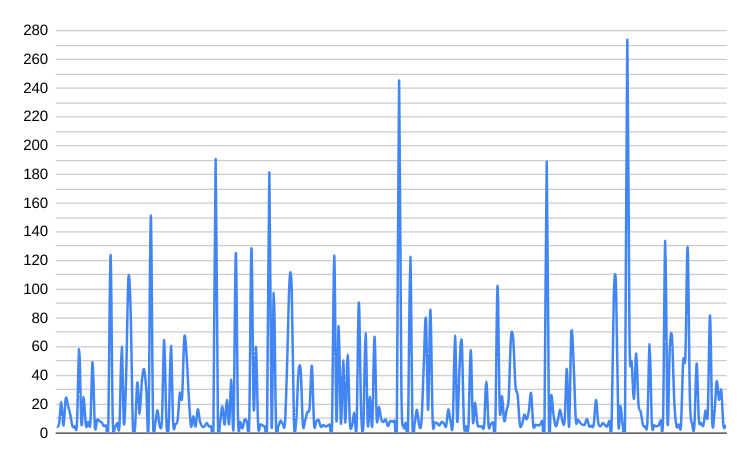
\includegraphics[scale=0.6]{graph}
\end{center}

	Проанализировав данный график, можно сделать выводы о характере заданной числовой последовательности:
\begin{itemize}
	\item Не является возрастающей/невозрастающей
	\item Не является убывающей/неубывающей
	\item Не является периодической
\end{itemize}

Поскольку график значкений для заданной чисолвой последовательности не имеет выраженных черт для данных характеристик.

\newpage
\mysubsection{Посроение гистограммы частот}
\begin{center}
	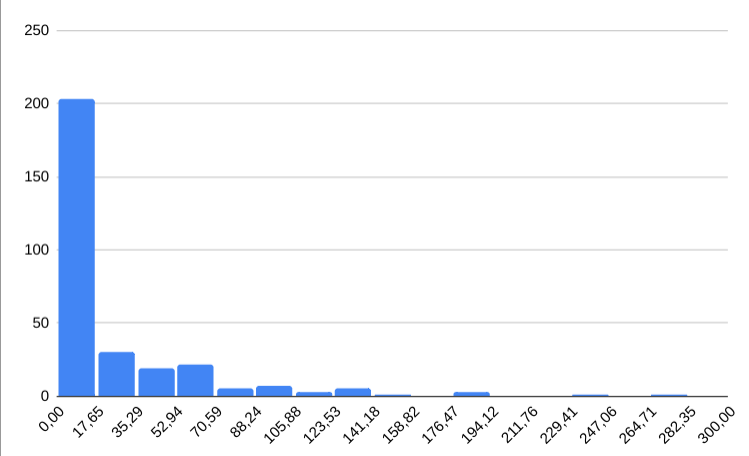
\includegraphics[scale=0.6]{histogram}
\end{center}

	Гистограмма дает представление функции плотности вероятности случайной величины, построенное по выборке. Можно сделать предположение, что заданная ЧП соотвествует закону гиперэкспоненциального распределения.

	Гистограмма имеет длинный хвост, что означает наличие редких экстремельных значений в последовательности, что характерно для гиперэкспоненциального распределения. Это означает что при гиперэкспоненциальном распределении вероятность появления больших значений случайной величины значительно выше, чем, например, для экспоненциального распредлеения.

	Также гистограмма гиперэкспоненциального распределения по сравнению с экспоненциальным распределением характеризуется более резким спадом в области малых занчений случайной величины, причем чем больше коэффициент вариации случайной величины, тем круче спад. Это значит, что вероятность появления маленьких значений случайной величины для гиперэкспоненциального распределения намного больше вероятности появления больших значений.
	
\newpage 

\mysubsection{Выполнение автокорреляционного анализа}
	Автокорреляция - это способ измерить, есть ли закономерность в последовательности. Она паказывает, насколько текущее значени данных связано с предыдущими значениями, можно ли зная текущее значение, предсказать предыдущее/следующее.
	
\begin{table}[h]
	\small
	\centering
	\begin{tabularx}{\textwidth}{| c | X | X | X | X | X | X | X | X | X | X | }
		\hline
		Сдвиг ЧП & 1 & 2 & 3 & 4 & 5 & 6 & 7 & 8 & 9 & 10 \\
		\hline
		К-т АК для заданной ЧП & -0,0131 & 0,0069 & -0,0969 & -0,0948 & -0,0109 & 0,0051 & -0,0003 & -0,0002 & 0,0846 & 0,0226  \\
		\hline
	\end{tabularx}
\end{table}

	Коэффициенты автокорреляции заданной числовой последовательности для 9 сдвигов меньше 0.1, что позволяет сказтаь, что последовательность случайна.

\mysubsection{Выполнение аппроксимации закона распределеиня}

	Рассчитанный коэффициент вариации случайной величины $v = 1,48 > 1$

	Для аппроксимации закона распределения такой случайной величины используют \textbf{гиперэкспоненциальной распределение}, представляющее собой композицию экспоненциальных распределений.

	Стоит отметить, что аппроксимация гиперэкспоненциального распределеиня может осуществляться по трем моментам распределения, так как оно является трехпараметрическим, т.е. содержит три независимых параметра. Таким обраом, имеется три параметра: q, t1, t2.

	По следующим формулам были рассчитаны три момента:

	Для аппроксимации закона распределения с коэффициентом вариации больше 1 двухфазным гиперэкспоненциальным распределением седует выбрать слудующее значение вероятности:
	\begin{center}
		$q \leq \frac{2}{1 + v^2} = 0,62688 $
	\end{center}

	Пусть $ q = 0.6 $ (вероятность формирования значения случайной величины в первой фазе), тогда математические ожидания первой и второй экспоненциальных фаз будут равны соотвественно рассчитанным t1 и t2:

	\begin{center}
		$t_1 = \left[1 + \sqrt{\frac{1 - q}{2q}(v^2 - 1)}\right] \cdot t = 42,348805$

		\vspace{0.5cm}

		$t_2 = \left[1 - \sqrt{\frac{q}{2(1 - q)}(v^2 - 1)}\right] \cdot t = 1,341817457$
	\end{center}

	Где t - математическое ожидание.


\newpage
\mysubsection{Реализация генератора случайных величин}

\newpage
\mysection{Выводы}
В рамках выполенной лабораторонй работы было проведено исследование числовой последовательности. Анализ последовательноси включал в себя оценку числовых моментов, а также коррекляционный анализ для выявления ее особенностей. Кроме того, проедпринимались попытки аппроксимации данной последовательности гиперэкспоненциальным законом распределения, основанным на трех чиловых моментах случайной величины.

Был написан код, гере.... (Вывод дописать)
\end{document}